\documentclass[aspectratio=169]{../latex_main/tntbeamer}  % you can pass all options of the beamer class, e.g., 'handout' or 'aspectratio=43'
\usepackage{dsfont}
\usepackage{bm}
\usepackage[english]{babel}
\usepackage[T1]{fontenc}
%\usepackage[utf8]{inputenc}
\usepackage{graphicx}
\graphicspath{ {./figures/} }
\usepackage{algorithm}
\usepackage[ruled,vlined,algo2e,linesnumbered]{algorithm2e}
\usepackage{hyperref}
\usepackage{booktabs}
\usepackage{mathtools}

\usepackage{amsmath,amssymb}

\DeclareMathOperator*{\argmax}{arg\,max}
\DeclareMathOperator*{\argmin}{arg\,min}

\usepackage{amsbsy}
\newcommand{\vect}[1]{\bm{#1}}
%\newcommand{\vect}[1]{\boldsymbol{#1}}

\usepackage{pgfplots}
\pgfplotsset{compat=1.16}
\usepackage{tikz}
\usetikzlibrary{trees} 
\usetikzlibrary{shapes.geometric}
\usetikzlibrary{positioning,shapes,shadows,arrows,calc,mindmap}
\usetikzlibrary{positioning,fadings,through}
\usetikzlibrary{decorations.pathreplacing}
\usetikzlibrary{intersections}
\pgfdeclarelayer{background}
\pgfdeclarelayer{foreground}
\pgfsetlayers{background,main,foreground}
\tikzstyle{activity}=[rectangle, draw=black, rounded corners, text centered, text width=8em]
\tikzstyle{data}=[rectangle, draw=black, text centered, text width=8em]
\tikzstyle{myarrow}=[->, thick, draw=black]

% Define the layers to draw the diagram
\pgfdeclarelayer{background}
\pgfdeclarelayer{foreground}
\pgfsetlayers{background,main,foreground}

% Requires XeLaTeX or LuaLaTeX
%\usepackage{unicode-math}

\usepackage{fontspec}
%\setsansfont{Arial}
\setsansfont{RotisSansSerifStd}[ 
Path=../latex_main/fonts/,
Extension = .otf,
UprightFont = *-Regular,  % or *-Light
BoldFont = *-ExtraBold,  % or *-Bold
ItalicFont = *-Italic
]
\setmonofont{Cascadia Mono}[
Scale=0.8
]

% scale factor adapted; mathrm font added (Benjamin Spitschan @TNT, 2021-06-01)
%\setmathfont[Scale=1.05]{Libertinus Math}
%\setmathrm[Scale=1.05]{Libertinus Math}

% other available math fonts are (not exhaustive)
% Latin Modern Math
% XITS Math
% Libertinus Math
% Asana Math
% Fira Math
% TeX Gyre Pagella Math
% TeX Gyre Bonum Math
% TeX Gyre Schola Math
% TeX Gyre Termes Math

% Literature References
\newcommand{\lit}[2]{\href{#2}{\footnotesize\color{black!60}[#1]}}

%%% Beamer Customization
%----------------------------------------------------------------------
% (Don't) Show sections in frame header. Options: 'sections', 'sections light', empty
\setbeamertemplate{headline}{empty}

% Add header logo for normal frames
\setheaderimage{
	% 
\includegraphics[height=\logoheight]{figures/TNT_darkv4.pdf}
	
\includegraphics[height=\logoheight]{../latex_main/figures/luh_logo_rgb_0_80_155.pdf}
	% 
\includegraphics[height=\logoheight]{figures/logo_tntluh.pdf}
}

% Header logo for title page
\settitleheaderimage{
	% 
\includegraphics[height=\logoheight]{figures/TNT_darkv4.pdf}
	
\includegraphics[height=\logoheight]{../latex_main/figures/luh_logo_rgb_0_80_155.pdf}
	% 
\includegraphics[height=\logoheight]{figures/logo_tntluh.pdf}
}

% Title page: tntdefault 
\setbeamertemplate{title page}[tntdefault]  % or luhstyle
% Add optional title image here
%\addtitlepageimagedefault{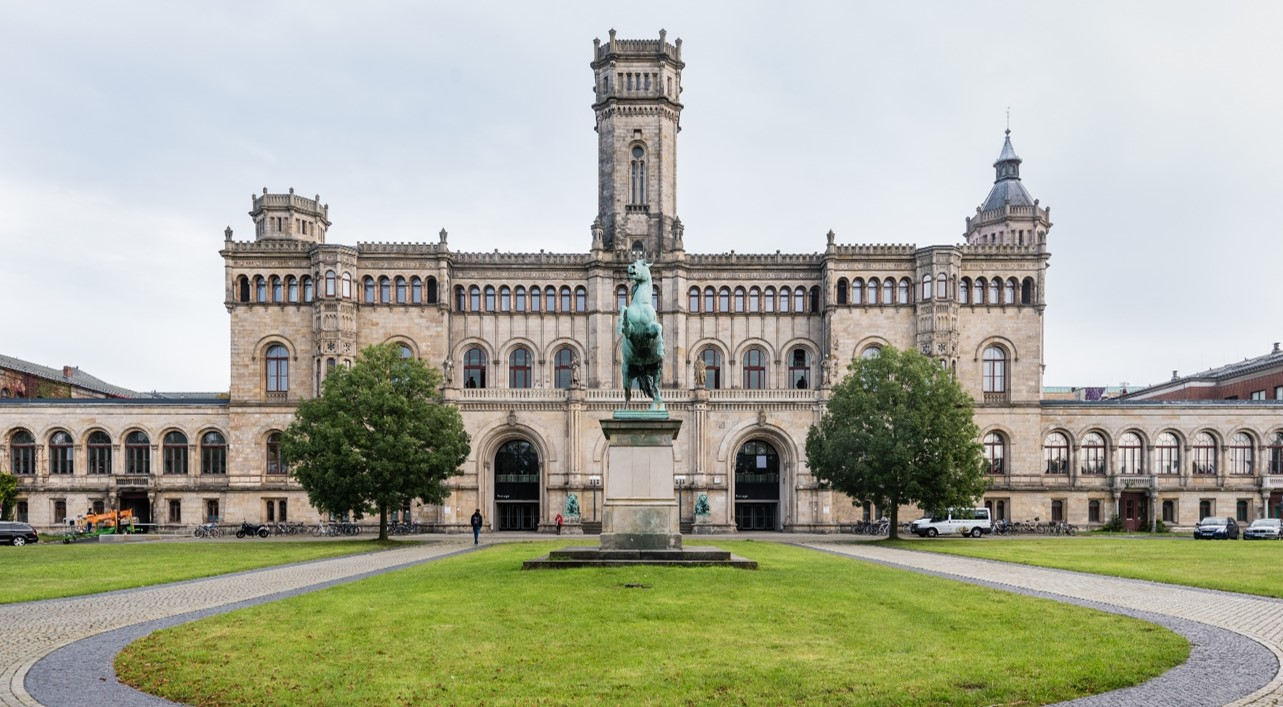
\includegraphics[width=0.65\textwidth]{figures/luh_default_presentation_title_image.jpg}}

% Title page: luhstyle
% \setbeamertemplate{title page}[luhstyle]
% % Add optional title image here
% \addtitlepageimage{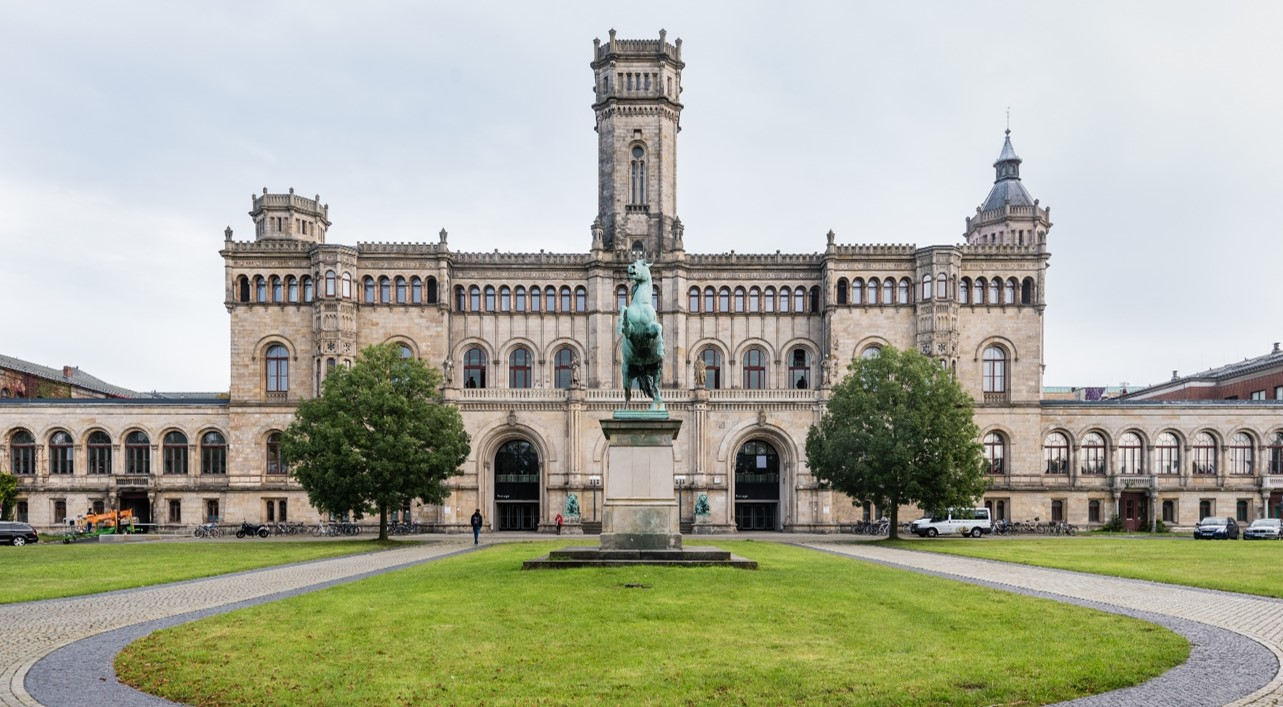
\includegraphics[width=0.75\textwidth]{figures/luh_default_presentation_title_image.jpg}}

\author[Abedjan \& Lindauer]{Ziawasch Abedjan \& Marius Lindauer\\[1em]
	
\includegraphics[height=\logoheight]{../latex_main/figures/luh_logo_rgb_0_80_155.pdf}\qquad
	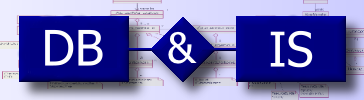
\includegraphics[height=\logoheight]{../latex_main/figures/DBIS_Kurzlogo.png}\qquad

\includegraphics[height=\logoheight]{../latex_main/figures/TNT_darkv4}\qquad

\includegraphics[height=\logoheight]{../latex_main/figures/L3S.jpg}	}
\date{Summer Term 2022; \hspace{0.5em} {
\includegraphics[height=1.5em]{../latex_main/figures/Cc-by-nc-sa_icon.svg.png}}; based on \href{https://ds100.org/fa21/}{[DS100]}
}


%%% Custom Packages
%----------------------------------------------------------------------
% Create dummy content
\usepackage{blindtext}

% Adds a frame with the current page layout. Just call \layout inside of a frame.
\usepackage{layout}


%%% Macros
%\renewcommand{\vec}[1]{\mathbf{#1}}
% \usepackage{bm}
%\let\vecb\bm

\title[Learning]{DS: Learning}
\subtitle{Learning Paradigms}

\graphicspath{ {./figure/} }
%\institute{}


\begin{document}
	
    \maketitle
    
    \begin{frame}[c]{What is machine learning?}

            Given
            \begin{itemize}
                \item Data distribution $\mathrm{P}$
                %\item paradigm $\mathcal{P}$
                \item loss function $\mathcal{L}$
            \end{itemize}
            find the best model $f^{\text{ }\ast}$ that minimizes the error:

            \begin{equation}
                f^{\text{ }\ast} \in \argmin_{f \in \mathcal{F}} \int_{x,y \sim \mathrm{P}} \mathcal{L}(f(x), y)
            \end{equation}

        Remarks:
        \begin{itemize}
            \item Solution might not be unique.
            \item Some people also like to use $h$ as a hypothesis from an hypothesis space
        \end{itemize}
        
    \end{frame}

    \begin{frame}[c]{Training}

        \begin{itemize}
            \item \alert{Overall Objective:} Identify patterns in training data that allow us to generalize to new data
            \bigskip
            \item \alert{Notes:} 
            \begin{itemize}
                \item The amount of data we collect is finite and thus, we will never cover all possible cases
                \item[$\leadsto$] We learn only an approximation of the real world
                \item[$\leadsto$] Approximation also helps us to focus on the important aspects and to filter noise in our observations
            \end{itemize}

            \item \alert{Learning} describes the process of going from a finite training dataset $\mathcal{D}$ to a learned model $\hat{f}$
            
        \end{itemize}
        
    \end{frame}

    \begin{frame}[c]{Learning Paradigms}

        \begin{itemize}
            \item \alert{Question}: What kind of training data is available?
            \begin{description}
                \item[$x,y$ pairs] $\leadsto$ supervised learning\newline $\leadsto$ you have a teacher that showed you the correct answers, and you were able to learn from it
                \item[$x$ but not $y$] $\leadsto$ unsupervised learning\newline $\leadsto$ you have many tasks, but no one telling you what is right and what is wrong\newline $\leadsto$ you have to discover the patterns yourself
                \item [$x$ and some $y$] $\leadsto$ semi-supervised learning\newline
                                         $\leadsto$ even unlabeled data points $x$ can help you to learn and infer some of the missing $y$~s
                \item[some $y$ but not $x$] $\leadsto$ recommendation system \newline
                                        $\leadsto$ Learn how different $y$~s relate to each other (e.g., product recommendation)
                \item[ $x$ can only be queried and some reward $r$] $\leadsto$ Reinforcement learning \newline
                    $\leadsto$ you can only learn by interacting with the environment
            \end{description}
            
        \end{itemize}
        
    \end{frame}

    \begin{frame}[c]{Identify Paradigms}

        \begin{itemize}
            \item In $90\%$ of all cases, you can identify the correct paradigm by the available data
            \item \alert{Pitfalls}:
            \begin{enumerate}
                \item For training, you have different kind of data than for deployment.
                \item Your training data is not informative, e.g., all data points have the same label $y$
                \item For all paradigms, there are different loss functions. The ``correct'' one might be needed to learn a good model (e.g., unbalanced data).
                \item Some learning algorithms have assumptions. Without knowing and considering these, the training can fail or generalization performance to new data can be horrible.
            \end{enumerate}
        \end{itemize}

        $\leadsto$ A good data scientist will be aware of these pitfalls, the corresponding solutions, and much more.
        
    \end{frame}


\end{document}